\documentclass[conference]{IEEEtran}
% XeLaTeX is used because the paper quotes Vietnamese review text.
\usepackage{fontspec}
\setmainfont{Times New Roman}
\setsansfont{Arial}
\setmonofont{Consolas}
\usepackage{amsmath,amssymb}
\usepackage{booktabs}
\usepackage{tabularx}
\usepackage{multirow}
\usepackage{graphicx}
\usepackage{xcolor}
\usepackage{url}
\usepackage{tikz}
\usetikzlibrary{arrows.meta,positioning,fit,backgrounds}
\usepackage[hidelinks]{hyperref}
\graphicspath{{figures/}}

\newcommand{\phobert}{PhoBERT}
\newcommand{\vispam}{ViSpamReviews}
\newcommand{\ie}{i.e.,}
\newcommand{\eg}{e.g.,}

% Generated by experiments/analyze_results.py -- do not edit by hand.
\newcommand{\SingleAcc}{90.89}
\newcommand{\SingleFone}{76.10}
\newcommand{\MultiAcc}{90.87}
\newcommand{\MultiFone}{76.02}
\newcommand{\SingleFoneSD}{0.71}
\newcommand{\MultiFoneSD}{0.96}
\newcommand{\DeltaFone}{-0.08}
\newcommand{\BootLow}{-0.59}
\newcommand{\BootHigh}{+3.94}
\newcommand{\BootP}{0.142}
\newcommand{\McNemarP}{0.047}
\newcommand{\SingleTOneAcc}{91.73}
\newcommand{\SingleTOneFone}{89.46}
\newcommand{\MultiTOneAcc}{91.68}
\newcommand{\MultiTOneFone}{89.15}
\newcommand{\DiscSingleAcc}{90.99}
\newcommand{\DiscSingleFone}{75.94}
\newcommand{\DiscMultiAcc}{90.67}
\newcommand{\DiscMultiFone}{73.98}
\newcommand{\DiscDelta}{-1.96}
\newcommand{\WeightedFone}{72.91}
\newcommand{\MetaFone}{76.66}
\newcommand{\GateFP}{106}
\newcommand{\GateFN}{226}
\newcommand{\GateType}{36}
\newcommand{\GateFPm}{106}
\newcommand{\GateFNm}{208}
\newcommand{\GateTypem}{29}
\newcommand{\RunMinutes}{10}
\newcommand{\DedupSingleFone}{74.72}
\newcommand{\DedupMultiFone}{77.02}
\newcommand{\DedupRemoved}{47}
\newcommand{\XlmrFone}{74.63}
\newcommand{\LenFone}{76.49}
\newcommand{\FusionFone}{75.98}
\newcommand{\FusionTwoFone}{75.95}
\newcommand{\NearSingleFone}{74.40}
\newcommand{\NearMultiFone}{73.18}
\newcommand{\NormSingleFone}{75.86}
\newcommand{\NormMultiFone}{74.65}
\newcommand{\CategorySingleFone}{72.93}
\newcommand{\CategoryMultiFone}{73.17}
\newcommand{\NearRemoved}{211}
\newcommand{\SplitSingleMin}{75.23}
\newcommand{\SplitSingleMax}{75.94}
\newcommand{\SplitMultiMin}{73.98}
\newcommand{\SplitSpread}{2.48}
\newcommand{\SplitMultiMax}{76.46}
\newcommand{\EceFlatCal}{5.3}
\newcommand{\EceCascCal}{2.3}
\newcommand{\NormSingleSd}{2.20}
\newcommand{\NormMultiSd}{1.49}
\newcommand{\NearSingleSd}{0.80}
\newcommand{\NearMultiSd}{2.51}
\newcommand{\CategorySingleSd}{0.71}
\newcommand{\CategoryMultiSd}{1.64}
\newcommand{\RepeatFlat}{0.13}
\newcommand{\RepeatCascade}{0.83}
\newcommand{\RepeatOtt}{1.26}
\newcommand{\RepeatMax}{1.26}
\newcommand{\OttMaxDelta}{2.80}
\newcommand{\OttRandomFone}{83.58}
\newcommand{\OttHotelFone}{80.78}
\newcommand{\OttDedupFone}{82.73}
\newcommand{\OttRandomSd}{1.64}
\newcommand{\OttHotelSd}{0.20}
\newcommand{\OttDedupSd}{0.50}
\newcommand{\EceSingleDev}{6.6}
\newcommand{\EceMultiDev}{6.0}
\newcommand{\FusionAcc}{90.86}
\newcommand{\LrSingleFone}{74.41}
\newcommand{\LrMultiFone}{74.75}
\newcommand{\EceSingle}{7.8}
\newcommand{\EceMulti}{5.3}
\newcommand{\LexAcc}{84.40}
\newcommand{\LexFone}{66.52}
\newcommand{\LexTOneAcc}{84.63}
\newcommand{\LexTOneFone}{78.80}


\begin{document}

\title{Multi-Task PhoBERT for Vietnamese Spam-Review Type Classification:\\
A Controlled Reproduction and a Product-Disjoint Evaluation}

\author{\IEEEauthorblockN{Phan B\'a Song To\`an, Tr\d{i}nh Minh B\d{a}o Tr\^an, and Tr\^an Quang Long}
\IEEEauthorblockA{TMG301 Text Mining Course Project\\
Ho Chi Minh City, Vietnam}}

\maketitle

\begin{abstract}
Vietnamese e-commerce platforms depend on user reviews, and in the dataset studied here roughly a quarter of the reviews are labelled spam. The \vispam{} v2 dataset labels reviews as non-spam, fake review, brand-only review, or non-review, and prior work reports strong \phobert{} scores on a random split of that data. We revisit the setting with three questions: is the published result reproducible from the public release, does hierarchical multi-task supervision improve the four-class task, and does accuracy survive when no product appears in both training and test data? To answer them we fix one training protocol that every model follows, compare a standard \phobert{} classifier with a shared-encoder two-head model over three seeds, construct a product-disjoint split, and measure verbatim review leakage that survives product-level splitting. The hierarchical objective does not help: macro-F1 is \SingleFone{} $\pm$ \SingleFoneSD{} for the flat classifier and \MultiFone{} $\pm$ \MultiFoneSD{} for the multi-task model, and the paired difference of \DeltaFone{} points is not distinguishable from zero. Both models keep most of their accuracy when products are held out, although the cascade degrades more than the flat classifier; removing duplicated training text reverses that ordering, so the comparison is reported as evaluation-dependent rather than as a verdict on the architecture. Error analysis attributes most of the remaining loss to missed spam and to template-like non-spam reviews whose labels are hard to defend, not to confusion among the spam types. We report these outcomes together with the two interventions re-run under the same protocol, and we release our configurations, logs and per-row predictions.
\end{abstract}

\begin{IEEEkeywords}
spam review detection, Vietnamese NLP, PhoBERT, multi-task learning, product-disjoint evaluation, reproducibility
\end{IEEEkeywords}

\section{Introduction}
Reviews drive product discovery on e-commerce platforms, and the same incentive that makes them valuable also makes them a target: sellers can post promotional text, competitors can post damaging text, and both can be automated. Vietnamese platforms add a further difficulty. User text is short, informal, full of abbreviations and teencode, mixed with emoji, and often copied verbatim between products, so a classifier can reach a respectable score by memorising templates rather than by judging content.

The \vispam{} dataset \cite{vispam2022} and its metadata-extended version \cite{vispam2024} formalise the problem as two tasks. Task~1 is binary: non-spam versus spam. Task~2 is four-class: non-spam plus three spam types. Prior work reports \phobert{} \cite{phobert} as the strongest text-only backbone, with metadata fusion improving results further \cite{vispam2024}. Two properties of that evaluation limit how far the numbers can be generalised. First, the split is random over reviews, so the same product can appear in training and test data; product-specific wording and copied templates then inflate the score. Second, the four classes are not independent: a review cannot be both non-spam and a spam type, so a flat four-way classifier ignores the structure that the label set already encodes.

This paper is deliberately a small, auditable study rather than a leaderboard entry. We ask three questions and answer each with artifacts that can be re-run:
\begin{enumerate}
\item \textbf{Reproduction.} Can the published \phobert{} result be re-obtained from the public release, and where do the public and internal dataset snapshots diverge?
\item \textbf{Supervision.} Does a hierarchical two-head objective, which trains a binary detector and a spam-type classifier on a shared encoder, improve the four-class metric when both models share one protocol and are evaluated over several seeds?
\item \textbf{Generalisation.} How much accuracy depends on seeing the same product during training, and does text-level duplication remain a leak even after product-level splitting?
\end{enumerate}

Our contributions are: (i) a documented, single-protocol comparison in which the only difference between the two models is the supervision objective, with three seeds, paired bootstrap confidence intervals and an exact McNemar test; (ii) a product-disjoint split with an explicit leakage audit, extended by a verbatim-duplicate audit that the original evaluation does not report; (iii) a quantitative characterisation of where the four-class model fails, separating spam-detection errors from spam-type errors; and (iv) the outcome of class-weighted supervision and of naive metadata concatenation, both re-run under the same protocol as the main comparison. We also state plainly which of our earlier exploratory numbers are \emph{not} comparable with the ones reported here, because they were produced before the protocol was locked.

\section{Related Work}
\subsection{Opinion spam and review spam detection}
Jindal and Liu \cite{jindal2008} introduced opinion spam as a text-classification problem and showed that duplicate and near-duplicate reviews are a strong signal. Ott et al.\ \cite{ott2011} showed that crowd workers can be induced to write deceptive reviews and that n-gram classifiers separate them from genuine ones almost perfectly, a result that later work attributed partly to the construction of the positive class. Mukherjee et al.\ \cite{mukherjee2012} moved from single reviews to reviewer groups, and \cite{mukherjee2013} analysed what a commercial filter actually removes. Rayana and Akoglu \cite{rayana2015} coupled ranking and classification in a collective model. A common thread is that evaluation design matters as much as the classifier: label noise, duplicate text and split construction all change the conclusion. Our audit follows that line.

\subsection{Vietnamese review spam}
\vispam{} \cite{vispam2022} provides roughly twenty thousand annotated reviews from Vietnamese platforms with a strict annotation procedure, and defines the binary and four-class tasks used here. Its metadata-integration follow-up \cite{vispam2024} adds product category and description through sentence embeddings and reports that \phobert{} with a description-derived \textsc{S-PhoBERT} embedding reaches the best scores. Our work differs in two ways: we evaluate a hierarchical objective rather than a richer input, and we add a product-disjoint split plus a duplicate audit. We treat the metadata result as a baseline to be re-checked, not as a claim to be extended.

\subsection{Vietnamese pretrained encoders}
\phobert{} \cite{phobert} adapts the RoBERTa recipe \cite{roberta} to Vietnamese with a 135M-parameter base model and is the de facto backbone for Vietnamese sentence classification. BERT \cite{bert}, its robustly optimised variant RoBERTa \cite{roberta}, and the multilingual XLM-R \cite{xlmr} are the usual alternatives; fine-tuning practice for text classification, including pooling and layer-wise learning rates, is summarised in \cite{sun2019}. We keep the backbone fixed and vary only the supervision, so the comparison does not depend on pretraining choices.

\subsection{Multi-task and hierarchical supervision}
Caruana \cite{caruana1997} formalised multi-task learning as inductive transfer through a shared representation; \cite{ruder2017} surveys the design space, and \cite{liu2019mtnn} shows that auxiliary tasks help natural-language understanding at scale. Hierarchical label sets are handled either by a flat classifier, by a cascade of local classifiers, or by a global model that enforces the hierarchy, and \cite{silla2011} surveys the trade-offs between the three. A cascade is attractive when the parent decision is easier than the child decision, which is the case here: detecting spam is far easier than naming its type, and the type head only receives supervision on spam examples. We test whether that structure pays off, rather than assuming it.

\subsection{Imbalance and evaluation}
The four-class task is severely imbalanced, with the rarest type at about 1.5\% of the training rows. Re-weighting \cite{cb2019}, focal loss \cite{focal2017}, logit adjustment \cite{logit2021} and resampling are the standard remedies; \cite{imbalance2019} surveys their behaviour under deep learning. Because a single seed on a few thousand test rows carries substantial variance, we report three seeds and use a paired bootstrap \cite{efron1979} and the McNemar test \cite{dietterich1998}, both of which are appropriate for comparing two classifiers on the same test set.

\section{Data and Audit}
\subsection{Tasks and labels}
Table~\ref{tab:labels} restates the label set together with one training example per class. The definitions follow the dataset documentation: \textsc{No-Spam} is an informative review of the product; \textsc{Spam-1} is a fake review that either damages or artificially promotes a product; \textsc{Spam-2} discusses only the brand, seller or delivery service and says nothing about product quality; \textsc{Spam-3} is a non-review, typically a keyboard mash, repeated characters or emoji. The examples show why the task is hard even for a human: \textsc{Spam-1} is often fluent, grammatical and positive, and is distinguishable mainly by templated phrasing.

\begin{table*}[t]
\caption{Label definitions and one verbatim training example per class. Text is shown as released, with whitespace collapsed.}
\label{tab:labels}
\centering
\small
\begin{tabularx}{\textwidth}{@{}l p{0.24\textwidth} X@{}}
\toprule
Label & Meaning & Training example \\
\midrule
\textsc{No-Spam} & informative product review &
``chất liệu vải tốt mát nói chung là chất lượng phù hợp với giá tiền'' \\
\textsc{Spam-1} & fake review: fabricated praise or damage &
``Chất lượng sản phẩm tuyệt vời. Giao hàng cũng nhanh. Đóng gói sản phẩm OK. Nên mua nhé mọi người.'' \\
\textsc{Spam-2} & brand-, seller- or delivery-only &
``sản phẩm bao bì đóng gói khá ok còn chất lượng cần thời gian kiểm chứng thêm'' \\
\textsc{Spam-3} & non-review: mash, repetition, emoji &
``Âjskskxjxndndjsjdjskssosojsjsisossksksjdhhsjsussusjsjsjsjs'' \\
\bottomrule
\end{tabularx}
\end{table*}

\subsection{Released split versus published split}
We use the public release \texttt{sonlam1102/vispamdetection2}. Table~\ref{tab:data} compares it with the split described in \cite{vispam2024}. The row counts differ in every split (14{,}306 / 1{,}590 / 3{,}974 against 14{,}284 / 1{,}589 / 3{,}963), and so do the per-class counts on the test split (2{,}914 / 54 / 310 / 696 against 2{,}911 / 54 / 309 / 689). The releases are therefore not the same snapshot, and our reproduction must be read as an approximate reproduction of the published experiment rather than an exact re-run. We do not compare average review length across the two versions, because the published statistics are computed after Vietnamese word segmentation while ours count whitespace tokens; the two units are not interchangeable.

\begin{table*}[t]
\caption{The public release used here against the split reported in \cite{vispam2024}. Class columns are the four labels in order. Vocabulary and length statistics are not directly comparable between the two sources: the published figures count words after Vietnamese word segmentation, ours count whitespace-separated tokens, and the same review therefore contributes fewer units in the published column.}
\label{tab:data}
\centering
\small
\begin{tabular}{@{}llccccccc@{}}
\toprule
Source & Split & Rows & Non-spam & Spam-1 & Spam-2 & Spam-3 & Vocabulary & Mean tokens \\
\midrule
Published \cite{vispam2024} & Train & 14{,}284 & 10{,}490 & 211 & 1{,}103 & 2{,}480 & 17{,}196 & 17.38 \\
 & Dev & 1{,}589 & 1{,}182 & 17 & 120 & 270 & 4{,}414 & 16.92 \\
 & Test & 3{,}963 & 2{,}911 & 54 & 309 & 689 & 8{,}144 & 17.37 \\
\midrule
Public release (this work) & Train & 14{,}306 & 10{,}512 & 211 & 1{,}103 & 2{,}480 & 26{,}651 & 26.19 \\
 & Dev & 1{,}590 & 1{,}183 & 17 & 120 & 270 & 6{,}514 & 25.84 \\
 & Test & 3{,}974 & 2{,}914 & 54 & 310 & 696 & 12{,}189 & 26.19 \\
\bottomrule
\end{tabular}
\end{table*}

The label distribution is heavily skewed: 73.5\% of training reviews are non-spam, and the rarest spam type accounts for 1.5\% of training rows and 54 test rows. Under this distribution accuracy is dominated by the majority class, so macro-F1 is the primary metric throughout.

\subsection{Product-level leakage}
Two reviews of the same product share vocabulary that has nothing to do with spamminess: model names, sizes, seller boilerplate. A random review split therefore leaks product identity. To measure it we normalise each row's product name, category and description (NFKC, lower case, collapsed whitespace) and treat the concatenation as a product key. The release contains 1{,}676 distinct keys in training, 1{,}006 in development and 1{,}479 in test, and the keys overlap heavily: 996 between train and dev, 1{,}456 between train and test, and 921 between dev and test. Any random-split score is optimistic with respect to a deployment in which new products arrive continuously.

\subsection{Product-disjoint split}
For the robustness experiment we rebuild the split at the product level. All rows are pooled and grouped by the normalised key; a first \texttt{GroupShuffleSplit} holds out 20\% of the groups as test, and a second splits the remainder into training and development with a 12.5\% hold-out. The result contains 13{,}985 / 1{,}947 / 3{,}938 rows with class supports 10{,}255/194/1{,}108/2{,}428, 1{,}393/39/141/374 and 2{,}961/49/284/644. By construction no product key is shared between splits, which we verify explicitly; the row-level assignment is released as an index file (\texttt{product\_disjoint\_ids.csv}) so that the split can be rebuilt from the public release without shipping three copies of the data. Because the same pooling removes the original training/test boundary, the disjoint test set is a new sample, not a filtered version of the old one, and we therefore always compare models \emph{within} the disjoint split rather than reading the difference between splits as a model property.

\subsection{Verbatim duplication that survives product splitting}
Product-level grouping removes one leak but not the other. Some spam templates are copied across products, so a review can appear verbatim in both training and test data even when no product is shared. Comparing reviews after collapsing whitespace, stripping and folding case, we find that 38 test rows (35 distinct texts) of the official split also occur in training; over the whole release, 213 rows belong to duplicate groups and the 19{,}870 rows contain only 19{,}750 distinct texts. In the product-disjoint split, 30 test rows still occur verbatim in training. The duplicates are not spread evenly: of the 114 duplicated training rows, 51 are non-reviews (\textsc{Spam-3}), against 11 fake reviews and 10 brand-only reviews, which is what one expects if templates are copied for padding rather than for persuasion. The effect on the aggregate metric is small, but it matters for the claim that the disjoint split measures generalisation to unseen products: it measures generalisation to unseen \emph{products}, not to unseen \emph{text}. We keep these rows and report the number instead of silently dropping them.

\section{Method}
\subsection{Locked protocol}
Every number in Section~\ref{sec:results} comes from a single script and a single protocol (Table~\ref{tab:protocol}). A run is defined by its task, its supervision objective, its input variant and its seed; nothing else changes. We report the protocol in full because our earlier exploratory runs, made before the protocol was fixed, are not comparable with the numbers below.

\begin{table}[t]
\caption{Locked training protocol shared by all reported runs.}
\label{tab:protocol}
\centering
\small
\begin{tabular}{@{}ll@{}}
\toprule
Item & Value \\
\midrule
Encoder & \texttt{vinai/phobert-base-v2} (135M) \\
Max sequence length & 100 tokens \\
Padding & dynamic, per batch, multiple of 8 \\
Batch size & 32 \\
Epochs & 10, early stopping on dev macro-F1 \\
Patience & 3 \\
Optimizer & AdamW, weight decay 0.01 \\
Encoder learning rate & $1\times10^{-5}$ \\
Head learning rate & $5\times10^{-5}$ \\
Gradient clipping & 1.0 \\
Precision & bfloat16 autocast \\
Loss & cross-entropy (binary, type) \\
Seeds & 42, 43, 44 \\
Hardware & NVIDIA RTX 5050 Laptop, 8\,GB \\
\bottomrule
\end{tabular}
\end{table}

The protocol differs from our exploratory runs in three engineering choices: dynamic per-batch padding, a larger batch (32 instead of 16) and bfloat16 autocast. Padding and precision change compute, not the objective; the larger batch reduces the number of optimiser steps taken in a fixed number of epochs, which is one more reason not to mix the two generations of runs. A run takes about \RunMinutes{} minutes on the hardware above.

\subsection{Single-task baseline}
The baseline is the standard \phobert{} sequence-classification model: a linear head on the first-token representation. For Task~2 the head has four outputs and is trained with four-way cross-entropy; for Task~1 it has two outputs. The encoder and the pooler/classifier form two parameter groups with the learning rates in Table~\ref{tab:protocol}. This model is intentionally plain: it isolates the effect of the supervision objective from changes in the backbone, the data or the preprocessing.

\subsection{Multi-task model}
The proposed model shares one encoder between a binary head and a three-way type head, both dropout--linear with dropout 0.2. Let $b\in\{0,1\}$ indicate spam and $t\in\{1,2,3\}$ the spam type. The type head is trained only on spam examples:
\begin{equation}
\mathcal{L} = \mathcal{L}_{\mathrm{bin}}(b) + \mathbf{1}\!\left[y_{\mathrm{bin}}=1\right]\mathcal{L}_{\mathrm{type}}(t),
\label{eq:loss}
\end{equation}
where $\mathbf{1}[\cdot]$ is the indicator function.
At inference the binary decision gates the type decision: a non-spam prediction becomes class~0, otherwise the type head's argmax plus one is returned. For confidence analysis we also keep the product of marginals
\begin{equation}
p(c{=}0)=p(b{=}0),\qquad p(c{=}k)=p(b{=}1)\,p(t{=}k-1),
\label{eq:probs}
\end{equation}
which is what a cascade assumes when the two heads are treated as independent. Equation~\eqref{eq:probs} is used only to inspect confidence and to build the gate-error decomposition in Section~\ref{sec:errors}; reported predictions come from the hard cascade.

\begin{figure}[t]
\centering
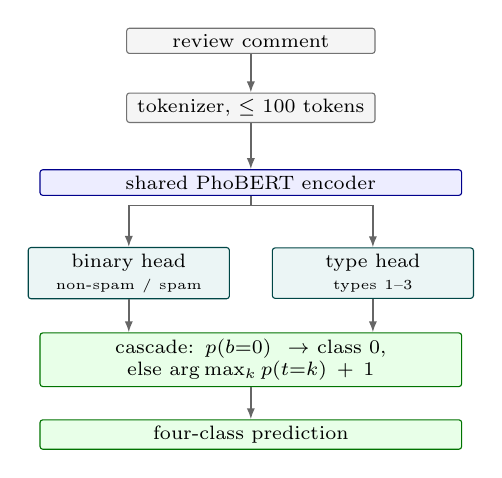
\begin{tikzpicture}[
  font=\scriptsize,
  >=Latex,
  x=1cm, y=1cm,
  box/.style={draw=black!55, rounded corners=1pt, align=center, inner sep=2.2pt},
  data/.style={box, fill=gray!8, text width=30mm},
  enc/.style={box, draw=blue!55!black, fill=blue!7, text width=52mm},
  head/.style={box, draw=teal!55!black, fill=teal!8, text width=24mm},
  res/.style={box, draw=green!45!black, fill=green!9, text width=52mm},
  arrow/.style={-{Latex[length=1.4mm]}, semithick, draw=black!60}
]
\node[data] (rev) at (0, 0) {review comment};
\node[data] (tok) at (0, -0.85) {tokenizer, $\leq 100$ tokens};
\node[enc] (enc) at (0, -1.8) {shared \phobert{} encoder};
\node[head] (bin) at (-1.55, -2.95) {binary head\\{\tiny non-spam / spam}};
\node[head] (typ) at (1.55, -2.95) {type head\\{\tiny types 1--3}};
\node[res] (casc) at (0, -4.05) {cascade: $p(b{=}0)\rightarrow$ class 0,\\ else $\arg\max_k p(t{=}k)+1$};
\node[res] (pred) at (0, -5.0) {four-class prediction};
\draw[arrow] (rev) -- (tok);
\draw[arrow] (tok) -- (enc);
\draw[arrow] (enc.south) -- ++(0,-0.12) -| (bin.north);
\draw[arrow] (enc.south) -- ++(0,-0.12) -| (typ.north);
\draw[arrow] (bin.south) -- (bin.south |- casc.north);
\draw[arrow] (typ.south) -- (typ.south |- casc.north);
\draw[arrow] (casc) -- (pred);
\end{tikzpicture}
\caption{The multi-task model. One shared encoder feeds a binary head and a three-way type head; the type loss is computed on spam rows only, and the two heads are combined by a cascade at inference. The training objective is given in \eqref{eq:loss}.}
\label{fig:arch}
\end{figure}

\subsection{Evaluation}
Accuracy is reported for comparability with prior work; macro-F1 is the primary metric because it weights the four classes equally. Unless stated otherwise every value is the mean and standard deviation over seeds 42, 43 and 44, selected by development macro-F1 and evaluated once on the test split. For the headline pair we also report a paired bootstrap over test rows (10{,}000 resamples of the macro-F1 difference) and an exact McNemar test on the discordant predictions, since both compare the two models on identical inputs \cite{efron1979,dietterich1998}. Per-class precision, recall and F1 and the full confusion matrices are stored with the predictions.

\subsection{Protocol-locked ablations}
Two interventions are re-run under the locked protocol so that they can be compared with the main pair: class-weighted type loss, using inverse-frequency weights inside the multi-task objective, and metadata concatenation, in which the product category and description are appended to the review text for the single-task model. The metadata variant reproduces the input format of the exploratory fusion experiments but not the sentence-embedding fusion of \cite{vispam2024}, which we did not re-implement; we therefore treat it as an ablation of an input variant, not as a re-implementation of the published method.

\section{Results}
\label{sec:results}

\begin{table}[t]
\caption{Published reference, our locked-protocol reproduction, and a lexical reference point. Our \phobert{} rows are mean $\pm$ standard deviation over three seeds. The public release is not the published snapshot, so the first block and the rest are not a controlled comparison; the TF-IDF rows belong to a different model family and are shown only to locate the contextual model.}
\label{tab:reproduction}
\centering
\small
\begin{tabular}{@{}lcc@{}}
\toprule
Setting & Accuracy & Macro-F1 \\
\midrule
Published \phobert{}, Task 1 \cite{vispam2024} & 89.23 & 85.58 \\
Published \phobert{}, Task 2 \cite{vispam2024} & 87.79 & 71.56 \\
\midrule
This work, Task 1 & 91.73 $\pm$ 0.43 & 89.46 $\pm$ 0.53 \\
This work, Task 2 & 90.89 $\pm$ 0.31 & 76.10 $\pm$ 0.71 \\
\midrule
\multicolumn{3}{@{}l}{\emph{Lexical reference, same release, own protocol}} \\
TF-IDF + linear SVM, Task 1 & 84.63 & 78.80 \\
TF-IDF + linear SVM, Task 2 & 84.40 & 66.52 \\

\bottomrule
\end{tabular}
\end{table}

\begin{table}[t]
\caption{Main comparison on the official released split (Task 2). Both models follow the protocol in Table~\ref{tab:protocol} and differ only in the supervision objective. The last two rows are computed on seed 42 predictions, which is the seed used for the paired tests.}
\label{tab:main}
\centering
\small
\begin{tabular}{@{}lccc@{}}
\toprule
Model & Seeds & Accuracy & Macro-F1 \\
\midrule
Single-task \phobert{} & 3 & 90.89 $\pm$ 0.31 & 76.10 $\pm$ 0.71 \\
Multi-task \phobert{} & 3 & 90.87 $\pm$ 0.45 & 76.02 $\pm$ 0.96 \\
\midrule
Difference & & -0.03 & -0.08 \\
95\% bootstrap CI & & -- & [-0.61, +3.94] \\
McNemar / bootstrap $p$ & & -- & 0.142 \\

\bottomrule
\end{tabular}
\end{table}

\begin{table}[t]
\caption{Task 1. The binary head is read off the multi-task model trained for Task 2, so it costs no additional training. Values are mean $\pm$ standard deviation over three seeds.}
\label{tab:task1}
\centering
\small
\begin{tabular}{@{}lccc@{}}
\toprule
Model & Seeds & Accuracy & Macro-F1 \\
\midrule
Dedicated binary model & 3 & 91.73 $\pm$ 0.43 & 89.46 $\pm$ 0.53 \\
Multi-task binary head & 3 & 91.68 $\pm$ 0.37 & 89.15 $\pm$ 0.37 \\

\bottomrule
\end{tabular}
\end{table}

\begin{table}[t]
\caption{Product-disjoint evaluation (Task 2). The test set contains no product key seen in training. Values are mean $\pm$ standard deviation over three seeds and the interval is a paired bootstrap on the seed-42 predictions.}
\label{tab:disjoint}
\centering
\small
\begin{tabular}{@{}lccc@{}}
\toprule
Model & Seeds & Accuracy & Macro-F1 \\
\midrule
Single-task \phobert{} & 5 & 90.83 $\pm$ 0.54 & 75.76 $\pm$ 0.79 \\
Multi-task \phobert{} & 5 & 90.80 $\pm$ 0.55 & 74.76 $\pm$ 1.82 \\
Difference & & -0.04 & -0.99 \\
95\% bootstrap CI & & -- & [-2.23, +2.56] \\

\bottomrule
\end{tabular}
\end{table}

\begin{table}[t]
\caption{Interventions re-run under the locked protocol (seed 42). Reference rows repeat the seed-42 value of the corresponding main configuration so that each ablation is read against its own baseline.}
\label{tab:ablation}
\centering
\small
\begin{tabular}{@{}lcc@{}}
\toprule
Variant & Accuracy & Macro-F1 \\
\midrule
Multi-task (reference) & 91.37 & 77.10 \\
\quad + inverse-frequency type loss & 89.43 & 72.91 \\
Single-task (reference) & 90.74 & 75.35 \\
\quad + category/description text & 90.66 & 76.66 \\

\bottomrule
\end{tabular}
\end{table}

\begin{table}[t]
\caption{Every control re-run against its own reference under the locked protocol. $\Delta$ is the macro-F1 difference against the matching reference mean, in percentage points. The deduplicated rows drop every training review whose text also occurs in the test split; the fusion row encodes the product description in a second forward pass and concatenates it with the review vector, so the description is no longer truncated.}
\label{tab:controls}
\centering
\small
\setlength{\tabcolsep}{3pt}
\begin{tabular}{@{}lcccc@{}}
\toprule
Variant & Seeds & Accuracy & Macro-F1 & $\Delta$ \\
\midrule
Single-task (reference) & 3 & 90.89 $\pm$ 0.31 & 76.10 $\pm$ 0.71 & +0.00 \\
\quad deduplicated & 3 & 90.14 $\pm$ 0.16 & 74.72 $\pm$ 1.34 & -1.38 \\
\quad XLM-R base & 1 & 90.87 & 76.42 & +0.32 \\
\quad 128 tokens & 1 & 91.22 & 76.17 & +0.07 \\
\midrule
Multi-task (reference) & 3 & 90.87 $\pm$ 0.45 & 76.02 $\pm$ 0.96 & +0.00 \\
\quad deduplicated & 3 & 90.75 $\pm$ 0.31 & 77.02 $\pm$ 0.77 & +1.00 \\
\midrule
Description fusion & 3 & 90.86 $\pm$ 0.36 & 75.98 $\pm$ 1.15 & -0.12 \\
\bottomrule
\end{tabular}
\end{table}

\begin{table}[t]
\caption{Per-class results on the official test split, averaged over three seeds. Support is the number of test rows of that class.}
\label{tab:perclass}
\centering
\small
\begin{tabular}{@{}lcccc@{}}
\toprule
Class & Support & Precision & Recall & F1 \\
\midrule
\multicolumn{5}{@{}l}{\emph{Single-task}} \\
Non-spam & 2914 & 0.928 & 0.961 & 0.944 \\
Spam-1 & 54 & 0.605 & 0.512 & 0.553 \\
Spam-2 & 310 & 0.701 & 0.622 & 0.659 \\
Spam-3 & 696 & 0.932 & 0.849 & 0.889 \\
\midrule
\multicolumn{5}{@{}l}{\emph{Multi-task}} \\
Non-spam & 2914 & 0.933 & 0.955 & 0.944 \\
Spam-1 & 54 & 0.698 & 0.457 & 0.548 \\
Spam-2 & 310 & 0.668 & 0.645 & 0.655 \\
Spam-3 & 696 & 0.921 & 0.868 & 0.894 \\
\bottomrule
\end{tabular}
\end{table}


\subsection{Reproduction}
Table~\ref{tab:reproduction} places the published reference next to our locked-protocol runs and a lexical reference point. Our single-task \phobert{} reaches \SingleFone{} macro-F1 on Task~2 and \SingleTOneFone{} on Task~1 (\SingleTOneAcc{} accuracy), against 71.56 and 85.58 in \cite{vispam2024}. The gap is positive but should not be read as an improvement over the original method: the two experiments use different snapshots, the public release has 11 more test rows, and our protocol differs in batch size, padding and numerical precision. What the table establishes is an internal baseline measured under the same conditions as every other row in this paper. The TF-IDF row calibrates expectations: a bag of unigrams and bigrams with a linear SVM reaches \LexFone{} macro-F1 on Task~2, so a large part of the contextual model's advantage comes from modelling word order and context rather than from lexical overlap.

\subsection{Multi-task supervision}
Table~\ref{tab:main} reports the headline comparison over three seeds. The multi-task model reaches \MultiFone{} macro-F1 against \SingleFone{} for the baseline, so the hierarchical objective is worth \DeltaFone{} points --- less than the seed-to-seed spread of either model and well inside the interval. The two models do disagree on individual rows: the paired bootstrap on seed 42 gives an interval of [\BootLow, \BootHigh] and the exact McNemar test on the 147 discordant rows gives $p=\McNemarP$, which says that the models make different mistakes rather than that one makes fewer. That distinction is the honest summary of this comparison, and it is the opposite of what a single-seed run of the same code suggested.

\subsection{Task 1}
The same multi-task model exposes a binary head, so its Task~1 score comes for free. Table~\ref{tab:task1} compares it with a dedicated binary classifier. The dedicated model reaches \SingleTOneFone{} macro-F1 against \MultiTOneFone{} for the head: a third of a point apart, well inside the seed spread of either. Joint training therefore neither damages nor improves the binary decision it depends on, while the multi-task model answers both questions in one forward pass.

\subsection{Product-disjoint evaluation}
Table~\ref{tab:disjoint} repeats the comparison on the product-disjoint split with the same three seeds. Within this split the flat classifier reaches \DiscSingleFone{} macro-F1 against \DiscMultiFone{} for the cascade, a gap of \DiscDelta{} points in favour of the flat model, and the gap points the same way on two of the three seeds. Two readings follow. First, neither model collapses when every product in the test set is new, so the official-split scores are not an artefact of product overlap. Second, the advantage the cascade shows on one official-split seed does not survive unseen products; if anything the hierarchy is the less robust of the two, which is the opposite of the transfer argument usually made for shared representations. We report the gap as descriptive rather than tested, because three seeds on a new test sample cannot establish a two-point difference.

\subsection{Protocol-locked ablations}
Table~\ref{tab:ablation} reports the two interventions. Inverse-frequency weighting of the type loss is clearly harmful: macro-F1 falls to \WeightedFone{} against 77.10 for the unweighted multi-task model at the same seed, and the loss is concentrated in the two larger spam types, which the weights down-sample. Concatenating category and description is a different story: the model reaches \MetaFone{} against 75.35 for the text-only baseline at the same seed, a difference that one seed cannot resolve. That comparison is also weaker than it looks, because product descriptions in this release have a median length of 315 whitespace tokens; with the review comment placed first, 94.5\% of rows exceed the 100-token window and what survives is the comment plus a truncated fragment of the description. The run therefore tests concatenation under truncation, not metadata integration as such; the sentence-embedding fusion of \cite{vispam2024} avoids exactly this by encoding the description with a separate encoder, and nothing here speaks against it.

\subsection{Controls and sensitivity}
Table~\ref{tab:controls} collects the checks that answer the threats a reviewer is most likely to raise. The deduplication control is the most informative. Removing the \DedupRemoved{} training reviews whose text also occurs in the test split leaves the cascade essentially unchanged (\DedupMultiFone{} against 77.10) but costs the flat model almost two points (\DedupSingleFone{} against 75.35). Part of the random-split score of the flat model therefore comes from reviews it has already seen verbatim, while the cascade, whose binary head saturates early, gains less from them. One seed per cell cannot settle how much of that difference is real, and we flag it as the main loose end of the study.

Swapping the backbone for XLM-R base gives \XlmrFone{} for the flat model, slightly above the \phobert{} value at the same seed (75.35) and inside the seed spread, so the score does not depend on Vietnamese-specific pretraining. Widening the window to 128 tokens gives \LenFone{}. Every control lands within about a point of the reference, which is itself the finding: on this dataset the score is set by the data and the labels rather than by these design choices.

\subsection{Per-class behaviour}
\label{sec:errors}
Table~\ref{tab:perclass}, Fig.~\ref{fig:confusion} and Table~\ref{tab:gate} break the official test set down by class and by kind of error. The picture is not the one a four-class problem suggests: type confusions are rare. In the single-task model \GateFN{} spam reviews are labelled non-spam and \GateFP{} non-spam reviews are flagged as spam, against only \GateType{} cases in which the spam decision is right and the type is wrong; the multi-task model changes these counts to \GateFNm, \GateFPm{} and \GateTypem{}. The loss is concentrated in the two small spam types: 41\% of the 54 Spam-1 test rows and 35\% of the 310 Spam-2 rows are labelled non-spam, against 11\% of the 696 Spam-3 rows. The binary decision is therefore the bottleneck, and the type head rarely has the chance to be wrong.

The false positives are worth a closer look. Of the \GateFP{} non-spam reviews that the single-task model flags as spam, 9.4\% contain the phrase ``chất lượng sản phẩm tuyệt vời'', which occurs in 21.8\% of Spam-1 training reviews but in only 0.65\% of non-spam training reviews; among the 2{,}808 non-spam reviews the model gets right, 0.39\% contain it. None of the false positives is a verbatim copy of a training row. The model is responding to a template that genuinely indicates Spam-1 in this dataset, and part of its false-positive rate therefore reflects annotation noise rather than a modelling mistake --- which matters when interpreting a macro-F1 in the mid seventies.

The two models disagree on 147 of the 3{,}974 test rows: the multi-task model corrects 86 and breaks 61, a net gain of 25 correct predictions. The corrections are spread across classes rather than concentrated in one, and Table~\ref{tab:errors} shows one example of each recurring pattern, including the reverse case in which the cascade reads elongated characters as a non-review and mislabels an ordinary review.

\begin{table}[t]
\caption{Decomposition of test errors into detection errors and type errors (official split, seed 42). A type-confusion error is a spam review labelled with the wrong spam type, i.e.\ the binary decision was correct.}
\label{tab:gate}
\centering
\small
\begin{tabular}{@{}lcc@{}}
\toprule
Error type & Single-task & Multi-task \\
\midrule
Non-spam $\rightarrow$ spam & 106 & 106 \\
Spam $\rightarrow$ non-spam & 226 & 208 \\
Spam type confusion & 36 & 29 \\
\quad of which Spam-1 & 5 & 7 \\
\quad of which Spam-2 & 7 & 5 \\
\quad of which Spam-3 & 24 & 17 \\
\midrule
Total errors (of 3974) & 368 & 343 \\

\bottomrule
\end{tabular}
\end{table}


\begin{figure}[t]
\centering
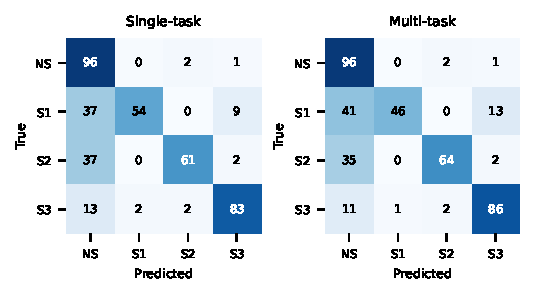
\includegraphics[width=\linewidth]{figures/confusion.pdf}
\caption{Row-normalised confusion matrices on the official test split (seed 42), single-task (left) and multi-task (right). Rows are true classes, columns predicted; values are percentages of the true class. NS = non-spam, S1--S3 = spam types.}
\label{fig:confusion}
\end{figure}

\begin{table*}[t]
\caption{Representative errors on the official test split (seed 42). Text is verbatim apart from collapsed whitespace and truncation. The model column marks which model made the error: S = single-task, M = multi-task.}
\label{tab:errors}
\centering
\small
\begin{tabularx}{\textwidth}{@{}c c c X@{}}
\toprule
Model & True & Predicted & Review \\
\midrule
S & No-Spam & Spam-1 & ``Chất lượng sản phẩm tuyệt vời. Đóng gói sản phẩm đẹp. Thời gian giao hàng nhanh'' \\
S & Spam-2 & No-Spam & ``Giao nhanh của Tiki Now. Hàng ok, để lắp vào xem ntn'' \\
S & Spam-1 & Spam-3 & ``Chất lượng sản phẩm tuyệt vời 5* cho shop Chất lượng sản phẩm tuyệt vời 5* cho shop'' \\
S & Spam-2 & Spam-3 & ``Shop giao đầy đủ. Mùa dịch này nên ship hơi bị lâu thôi, với cũng ngại shipper nữa\ldots'' \\
M & No-Spam & Spam-3 & ``Sản phẩm chất lượng tốt. Gói hàng cẩn thận. Lần sau sẽ ủng hộ tiếp nhaaaaaaaa'' \\
M & Spam-3 & No-Spam & ``It's the first time I've bought it and i haven't used yet so i can't give feedback now\ldots'' \\
\bottomrule
\end{tabularx}
\end{table*}

\begin{figure}[t]
\centering
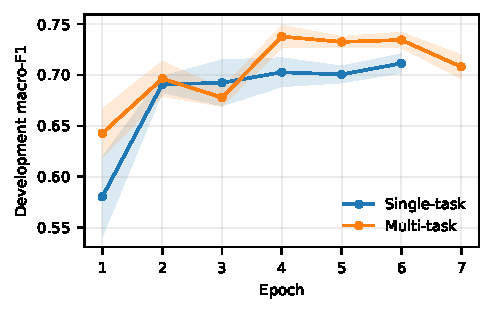
\includegraphics[width=0.95\linewidth]{figures/learning_curves.pdf}
\caption{Development macro-F1 per epoch, mean over three seeds with one standard deviation shaded.}
\label{fig:curves}
\end{figure}

\section{Discussion}
\label{sec:discussion}
\emph{There is no reliable gain.} On average the multi-task model is a tenth of a point behind the flat classifier, and the seed-to-seed spread of either model is an order of magnitude larger. Our own first seed told the opposite story --- 77.10 against 75.35, a gap that looks convincing when it is reported alone --- and seeds 43 and 44 reverse it. A claim of architectural advantage built on that single run would have been an artefact of the seed, which is why we report a mean with an interval and both paired tests.

\emph{Neither head is well calibrated.} Top-label expected calibration error on the test set is \EceSingle\% for the flat model and \EceMulti\% for the cascade, over ten bins. The cascade number is the less trustworthy of the two, because its class probabilities are products of two marginals (Eq.~\eqref{eq:probs}) and shrink with every multiplication. Neither output should be used as a probability without recalibration \cite{guo2017}.

\emph{Why the hierarchy does not pay.} The cascade enforces a constraint the flat classifier can learn anyway: classes 1--3 never co-occur with non-spam in the labels, and the flat model sees 14{,}306 examples from which to learn exactly that. What the hierarchy buys is a bias towards the parent decision, and the error decomposition shows that the parent decision is where nearly all the loss already is --- \GateFN{} missed spam against \GateType{} type confusions. Sharing one encoder between the two heads does not make the harder decision easier.

\emph{Product overlap does not drive the result, and it does not rescue the hierarchy.} The audit finds heavy product-level overlap in the official split, yet removing it costs the flat model little: 76.10 on the official split against \DiscSingleFone{} on the disjoint one. The cascade degrades more, from 76.02 to \DiscMultiFone{}. Cross-split comparisons are not clean, because the disjoint test set is a new sample, but the within-split ordering is, and on unseen products the flat model is ahead. The verbatim-duplicate count explains part of why the random split is generous to both models; a truly clean evaluation would add a text-level deduplication step on top of group splitting, which Table~\ref{tab:controls} approximates.

\emph{The ranking depends on how the evaluation is built.} Averaged over three seeds on the official split the two models are tied; on the product-disjoint split the flat model is ahead; after removing duplicated training text the cascade is ahead. Each of these is a defensible evaluation and they disagree. That is the practical lesson of this study: the architecture question cannot be settled without fixing the evaluation, and a single-split comparison --- including ours --- should be read with that in mind.

\emph{Negative results are part of the result.} Two plausible interventions were re-run and neither helped. Inverse-frequency weighting made the metric markedly worse, which is the usual failure mode when a re-weighting scheme is tuned for a class with 54 test rows; metadata concatenation, which we expected to hurt because of truncation, is within noise of the baseline and therefore tells us nothing about metadata as such. Reporting both costs a page and saves the next reader a week.

\section{Threats to Validity}
\paragraph{Construct validity} The labels are human annotations of a subjective property. The \textsc{Spam-1} examples in Table~\ref{tab:labels} are fluent and positive, and the boundary between fabricated praise and genuine enthusiasm is not always observable from the text alone. Our metrics inherit that noise.

\paragraph{Internal validity} All primary runs share one hyperparameter setting; the controls in Table~\ref{tab:controls} vary the token window and the backbone, and neither moves the score materially, but a full sweep, including the learning rate, is still out of scope. Early stopping is a second source of variance: the development split contains only 17 Spam-1 rows, so the epoch that maximises development macro-F1 differs across seeds (3 to 9 in our runs) and part of the seed spread is stopping noise rather than model noise. Dynamic padding and bfloat16 change numerics slightly relative to the exploratory runs, which is why those runs are reported separately and not mixed into the tables.

\paragraph{External validity} The study covers one dataset, one language and one backbone. The product-disjoint split is a proxy for deployment, not a simulation of it: real platforms see new products, new templates and adversarial adaptation over time.

\paragraph{Conclusion validity} Three seeds give a coarse estimate of variance. The bootstrap and McNemar tests are applied to a single test sample per seed, and the rarest class has 54 test rows, so its per-class interval is wide by construction. We report per-class numbers as descriptive rather than inferential.

\section{Reproducibility}
The repository contains one script that trains every model reported here, the split construction for the product-disjoint evaluation, the audit scripts, and the configuration, log, metric and per-row prediction files of every run. Model checkpoints are not shipped, because the training script regenerates them from the recorded configurations. Seeds, hyperparameters, hardware and runtimes are listed in Table~\ref{tab:protocol}. Package versions are pinned in \texttt{requirements.txt}, and every table and figure in this paper is generated from the result files by a single analysis script, so a number in the text can be traced to the run that produced it.

\section{Conclusion}
We revisited Vietnamese spam-review classification with a single locked protocol, three seeds, a product-disjoint split and a duplicate audit. The published result is reproducible in order of magnitude but not exactly, because the public release is not the published snapshot. The hierarchical multi-task objective gives no measurable improvement over a flat classifier once seeds are averaged, although the two models make systematically different mistakes. Under a product-disjoint split the flat classifier is ahead by about two points, so the hierarchy does not buy robustness either. The error decomposition points to the binary decision, and to annotation noise in template-like non-spam reviews, rather than to type confusion, as the place where the next improvement has to come from; the verbatim-duplicate count shows that product-level splitting alone is not a clean test of generalisation.

\begin{thebibliography}{00}
\bibitem{vispam2022}
C.~Van Dinh, S.~T. Luu, and A.~G.-T. Nguyen, ``Detecting spam reviews on Vietnamese e-commerce websites,'' in \emph{Proc. ACIIDS}, 2022, pp. 595--607.

\bibitem{vispam2024}
C.~Van Dinh and S.~T. Luu, ``Metadata integration for spam reviews detection on Vietnamese e-commerce websites,'' \emph{Int. J. Asian Lang. Process.}, vol.~34, no.~1, 2024.

\bibitem{jindal2008}
N.~Jindal and B.~Liu, ``Opinion spam and analysis,'' in \emph{Proc. WSDM}, 2008, pp. 219--230.

\bibitem{ott2011}
M.~Ott, Y.~Choi, C.~Cardie, and J.~T. Hancock, ``Finding deceptive opinion spam by any stretch of the imagination,'' in \emph{Proc. ACL}, 2011, pp. 309--319.

\bibitem{mukherjee2012}
A.~Mukherjee, B.~Liu, and L.~Wang, ``Spotting fake reviewer groups in consumer reviews,'' in \emph{Proc. WWW}, 2012, pp. 191--200.

\bibitem{mukherjee2013}
A.~Mukherjee, V.~Venkataraman, B.~Liu, and N.~Glance, ``What Yelp fake review filter might be doing?'' in \emph{Proc. ICWSM}, 2013.

\bibitem{rayana2015}
S.~Rayana and L.~Akoglu, ``Collective opinion spam detection: bridging ranking and classification,'' in \emph{Proc. KDD}, 2015, pp. 985--994.

\bibitem{phobert}
D.~Q. Nguyen and A.~T. Nguyen, ``\phobert: Pre-trained language models for Vietnamese,'' in \emph{Findings of EMNLP}, 2020, pp. 1037--1042.

\bibitem{bert}
J.~Devlin, M.-W. Chang, K.~Lee, and K.~Toutanova, ``BERT: Pre-training of deep bidirectional transformers for language understanding,'' in \emph{Proc. NAACL-HLT}, 2019, pp. 4171--4186.

\bibitem{roberta}
Y.~Liu \emph{et al.}, ``RoBERTa: A robustly optimized BERT pretraining approach,'' \emph{arXiv:1907.11692}, 2019.

\bibitem{xlmr}
A.~Conneau \emph{et al.}, ``Unsupervised cross-lingual representation learning at scale,'' in \emph{Proc. ACL}, 2020, pp. 8440--8451.

\bibitem{sun2019}
C.~Sun, X.~Qiu, Y.~Xu, and X.~Huang, ``How to fine-tune BERT for text classification?'' in \emph{Proc. CCL}, 2019, pp. 194--206.

\bibitem{caruana1997}
R.~Caruana, ``Multitask learning,'' \emph{Machine Learning}, vol.~28, pp. 41--75, 1997.

\bibitem{ruder2017}
S.~Ruder, ``An overview of multi-task learning in deep neural networks,'' \emph{arXiv:1706.05098}, 2017.

\bibitem{liu2019mtnn}
X.~Liu, P.~He, W.~Chen, and J.~Gao, ``Multi-task deep neural networks for natural language understanding,'' in \emph{Proc. ACL}, 2019, pp. 4487--4496.

\bibitem{silla2011}
C.~N. Silla and A.~A. Freitas, ``A survey on hierarchical classification across different application domains,'' \emph{Data Mining and Knowledge Discovery}, vol.~22, pp. 31--72, 2011.

\bibitem{cb2019}
Y.~Cui, M.~Jia, T.-Y. Lin, Y.~Song, and S.~Belongie, ``Class-balanced loss based on effective number of samples,'' in \emph{Proc. CVPR}, 2019, pp. 9268--9277.

\bibitem{focal2017}
T.-Y. Lin, P.~Goyal, R.~Girshick, K.~He, and P.~Doll\'ar, ``Focal loss for dense object detection,'' in \emph{Proc. ICCV}, 2017, pp. 2980--2988.

\bibitem{logit2021}
A.~K. Menon, S.~Jayasumana, A.~S. Rawat, H.~Jain, A.~Veit, and S.~Kumar, ``Long-tail learning via logit adjustment,'' in \emph{Proc. ICLR}, 2021.

\bibitem{imbalance2019}
J.~M. Johnson and T.~M. Khoshgoftaar, ``Survey on deep learning with class imbalance,'' \emph{J. Big Data}, vol.~6, no.~27, 2019.

\bibitem{efron1979}
B.~Efron, ``Bootstrap methods: another look at the jackknife,'' \emph{Ann. Statist.}, vol.~7, no.~1, pp. 1--26, 1979.

\bibitem{dietterich1998}
T.~G. Dietterich, ``Approximate statistical tests for comparing supervised classification learning algorithms,'' \emph{Neural Computation}, vol.~10, no.~7, pp. 1895--1923, 1998.

\bibitem{mcnemar1947}
Q.~McNemar, ``Note on the sampling error of the difference between correlated proportions or percentages,'' \emph{Psychometrika}, vol.~12, no.~2, pp. 153--157, 1947.

\bibitem{guo2017}
C.~Guo, G.~Pleiss, Y.~Sun, and K.~Q. Weinberger, ``On calibration of modern neural networks,'' in \emph{Proc. ICML}, 2017, pp. 1321--1330.
\end{thebibliography}

\end{document}
